\documentclass[10pt,a4paper]{article}
\usepackage[utf8]{inputenc}
\usepackage[T1]{fontenc}
\usepackage{lmodern}
\usepackage[margin=1.5cm, top=1.4cm, bottom=1.4cm]{geometry}
\usepackage{hyperref}
\usepackage{enumitem}
\usepackage{titlesec}
\usepackage{xcolor}
\usepackage{graphicx}

\definecolor{accent}{HTML}{00686E}
\hypersetup{colorlinks=true, urlcolor=accent, linkcolor=accent}
\pagenumbering{arabic}
\setlength{\parindent}{0pt}

\titleformat{\section}{\large\bfseries\color{accent}}{}{0em}{}[\vspace{-0.6em}\rule{\textwidth}{0.8pt}]
\titlespacing{\section}{0pt}{7pt}{4pt}

\newcommand{\role}[4]{%
  \textbf{#1} \hfill \textbf{#2}\\[1pt]%
  \textit{#3} \hfill \textit{#4}\\[2pt]%
}
\setlist[itemize]{leftmargin=1.2em, itemsep=1.5pt, topsep=2pt, parsep=0pt}

\begin{document}

% ================= HEADER =================
\begin{minipage}[c]{0.80\textwidth}
  {\Huge\bfseries Prabhavit Gupta}\\[3pt]
  {\color{accent}\large Senior Solutions Engineer: AI Search, Developer Platform \& API Integrations}\\[6pt]
  {\footnotesize +39 351 610 7807 ~$\vert$~
  \href{mailto:prabhavitg@gmail.com}{prabhavitg@gmail.com} ~$\vert$~
  \href{https://www.linkedin.com/in/prabhavit/}{linkedin.com/in/prabhavit} ~$\vert$~
  \href{https://github.com/prab-gupta}{github.com/prab-gupta} ~$\vert$~
  Venice, Italy}
\end{minipage}\hfill
\begin{minipage}[c]{0.18\textwidth}
  \raggedleft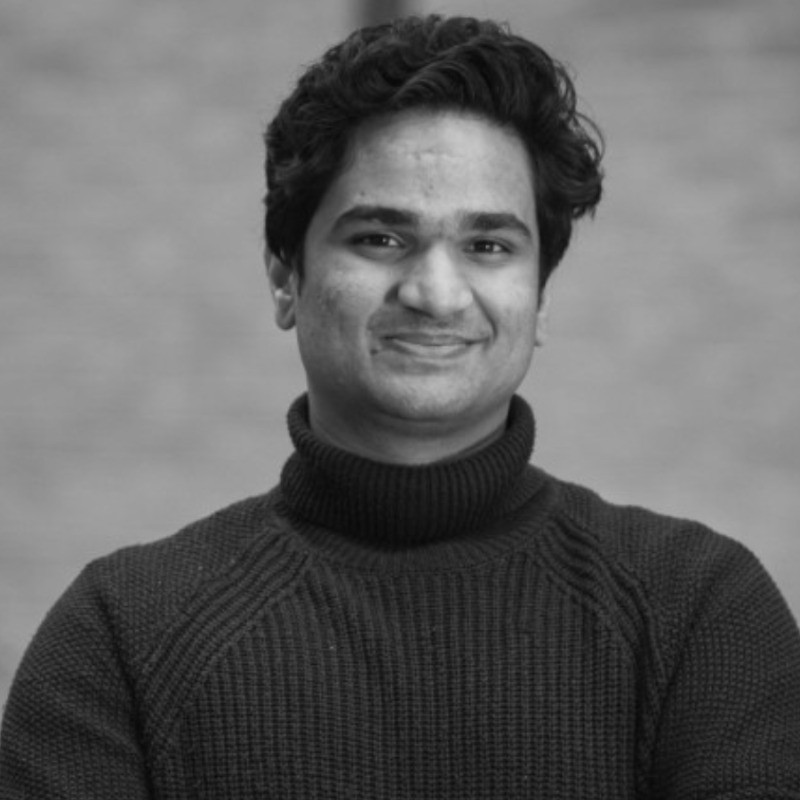
\includegraphics[width=2.0cm]{photo.jpg}
\end{minipage}
\vspace{-2pt}

% ================= SUMMARY =================
\section{Summary}
Solutions and Integration Engineer with 3 years of hands-on experience architecting production LLM agents, RAG retrieval pipelines, and developer-facing API integrations across European tech environments. At FlowSpace, engineered autonomous AI customer agents utilizing live API tool calling, structured JSON output schemas, and automated knowledge ingestion from heterogeneous documents across 900+ verified listings. Proficient in testing and demonstrating APIs with cURL, Postman, TypeScript, and working-level Python, translating developer needs into working proof-of-concepts, and bridging technical evaluation with commercial adoption. Experienced in lexical vs. semantic search, context management, and rate-limit handling across Claude, OpenAI, and Gemini ecosystems. Based in Venice, Italy with an EU Long Term Residence Permit (unrestricted EU work authorization without sponsorship). Immediately available.

% ================= TECHNICAL EXPERTISE =================
\section{Technical Expertise}
\begin{itemize}
  \item \textbf{AI \& Search Infrastructure:} RAG retrieval pipelines, Semantic vs. Lexical search, Context window optimization, LLM Tool/Function calling, Prompt engineering, Structured schemas, Anthropic Claude, OpenAI, Google Gemini.
  \item \textbf{API \& Developer Platform:} RESTful API design, cURL, Postman, Webhooks, Idempotency, Rate-limiting, Authentication patterns, Error budget handling, Developer documentation \& quickstarts.
  \item \textbf{Full Stack \& Prototyping:} TypeScript, JavaScript, Node.js, Working-level Python, Next.js, Supabase, PostgreSQL, Playwright, n8n, Docker, Git.
  \item \textbf{Solutions Engineering:} Technical discovery, Proof-of-concept (POC) builds, Interactive product demos, Developer advocacy, Customer requirement translation to Product/Engineering roadmaps.
  \item \textbf{Languages \& Work Authorization:} Hindi (Native), English (C1 Professional), Italian (Beginner). EU Long Term Residence Permit (Permanent unrestricted EU work authorization; no visa sponsorship required).
\end{itemize}

% ================= EXPERIENCE =================
\section{Experience}

\role{\href{https://flowspace.co}{FlowSpace.co}}{Mar 2024 - Aug 2026}{Lead Developer (Full-time, Freelance)}{London, UK (remote)}
\begin{itemize}
  \item Architected and shipped production AI agents using tool calling and live REST API function calling to query backend databases and trigger real-time bookings with fallback error handling.
  \item Built an automated knowledge ingestion pipeline: parsed heterogeneous documents (PDFs, spreadsheets, web pages) into structured database records using LLM extraction prompts, creating 900+ verified records.
  \item Engineered agentic developer workflows and internal tooling using Claude Code, TypeScript, and automated testing, accelerating feature delivery cycles across the engineering team.
  \item Conducted technical discovery with business partners and early adopters, building custom proof-of-concept integrations and demonstrating API capabilities.
  \item Integrated external partner REST APIs (OfficeRnD, Nexudus, Stripe) with idempotent event handling and automated webhook reconciliation.
  \item Implemented token tracking, prompt versioning, and end-to-end regression testing with Playwright to maintain high output fidelity across production agent runs.
  \item Directed platform architecture migration off a legacy stack to a modern Next.js, TypeScript, and Laravel backend, establishing reliable schema contracts and API specifications.
  \item Scaled platform user base from 2,000 to 4,500+ active users through iterative product engineering and resilient backend automations.
\end{itemize}

\role{Urlink}{Apr 2025 - Jul 2025}{Project Manager \& AI Assisted Developer (Freelance)}{Barcelona, Spain (remote)}
\begin{itemize}
  \item Led technical delivery of AI-assisted web applications, coordinating API contracts, database schemas, and external integrations.
  \item Evaluated commercial LLM APIs (OpenAI, Anthropic) across task types, optimizing prompt structures and model selection for latency and output consistency.
  \item Implemented automated CI/CD checks and test suites, ensuring clean code releases and minimal deployment regressions.
\end{itemize}

\role{Independent Technical Consultant}{Aug 2023 - Feb 2024}{AI Solutions \& Automation Engineer}{Venice, Italy}
\begin{itemize}
  \item Developed custom AI automations, agent prototypes, and data extraction pipelines for European SME clients using n8n, Playwright, and LLM APIs.
  \item Implemented idempotent webhook listeners and CRM data synchronization flows, replacing error-prone manual administrative processes.
  \item Built prototype RAG inquiry assistants integrated with company documentation for rapid customer response triage.
\end{itemize}

% ================= EDUCATION =================
\section{Education}
\role{Ca' Foscari University of Venice}{2020 - 2024}{BA in Philosophy, International Studies and Economics}{Venice, Italy}
\begin{itemize}
  \item In-depth focus on formal logic, analytical problem solving, systems analysis, and macroeconomic decision models.
\end{itemize}

\end{document}
